\subsection{\emph{Adaptative Contrast Enhancement}}

El método de \emph{Adaptative Contrast Enhancement} toma la técnica de
\emph{HE}, pero la aplica a diferentes regiones del histograma con el objetivo
de disminuir la distorsión generada por el método original. \\

\graficarMulticolPNG{claro_regions}{Diferenciación entre regiones de luminancia
en el histograma de la imagen.}{fig:regiones}

Se definen tres regiones de igual longitud en el histograma basadas en el nivel
de luminancia: oscuro, medio y claro (Figura \ref{fig:regiones}). El método
aplica un \emph{HE} independiente a cada región y luego las une, ponderándolas
según algún criterio a definir.\\

La realización de dicho criterio se encuentra en el factor $w_{i}$ definido para
cada región $i$. El uso de un vector de pesos $W = \begin{bmatrix} w_1 & w_2 & w_3 \end{bmatrix}$
trae dos ventajas fundamentales: mejoras personalizadas para cada caso
particular de imagen y la alternativa de modos de operación. Un caso de uso de los modos
de operación son los filtros provistos por las aplicaciones móbiles para retocar
imágenes para subirlas a las redes sociales. Las mismas aplicaciones suelen tener además
una opción para refinar la imagen de forma más detallada.\\

En el caso más genérico del método, los pesos son calculados a partir de la
pseudo varianza de cada región dadas las medias de luminancia
correspondientes. La varianza da una noción de la forma del histograma, en
particular denota si los puntos se encuentran concentrados en un rango pequeño
de valores o si están dispersos. Analíticamente obtenemos la pseudo varianza
$\sigma_i$ para cada región $i$ según:

\begin{equation} \label{eq:sigma}
	\sigma_i = \frac{1}{N_i} \sum_{j=0}^{m_i} h_j \cdot \left|y_j - \mu_i\right|
\end{equation}

donde, $N_i$ y $m_i$ son la cantidad de píxeles y la cantidad de niveles de
lumniancia dentro del rango $i$ respectivamente. Los valores $h_j$ corresponden
a la cantidad de píxeles cuyo nivel de luminancia es $y_j$ (equivalente al valor
del histograma para $j$). Por último, $\mu_i$ es la media de valores de
luminancia asociado al rango $i$.\\

Habiendo calculado la pseudo varianza para cada rango, se obtienen los pesos a
partir de la siguiente ecuación:

\begin{align} \label{eq:w}
	w_i &= \eta_i \left(1 - \left|\frac{2 \,\sigma_i}{\sigma_{\max}} -1 \right|\right) & \text{con }{\sigma_{\max} = \frac{\max\limits_{\forall j \in \, I}{y_j}}{2}}
\end{align}

con $\eta_i$ siendo un factor de forma determinado por el usuario para
refinamiento de la imagen. El valor de $\sigma_{\max}$ se halla a partir del
peor caso cuya distribución estaría concentrada sólo en los extremos de forma
equiprobable.\\

La ecuación \eqref{eq:w} nace del análisis de comportamiento esperado de los
pesos en función de la pseudo varianza. Para nuestra aplicación, buscamos
asignarle pesos mayores a aquellas regiones cuya pseudo varianza es moderada
porque esto implica que la ecualización generaría poca distorsión. En los casos
extremos (varianza máxima y mínima), la ecualización produciría grandes o nulos
cambios. Gráficamente, la función para calcular los pesos se encuentra en la
Figura \ref{fig:pesos}.

\graficarMulticolPNG{graph_weight_factor}{Función de pesos $w_i$ para cada valor de varianza.}{fig:pesos}

Una vez calculado el vector de pesos, se procede a realizar la ecualización
para cada región. Para ello, se comienza tomando los valores de la función
de densidad acumulada (\emph{CDF}) correspondientes a la región asociada. Luego,
basádonse en la ecuación \eqref{eq:he_full}, se hace el promedio ponderado entre
la ecualizada y la original para la región $i$-ésima según:

\begin{equation} \label{eq:ace}
	\textit{ACE}_i = \textit{orig}_i - w_i \left(\textit{orig}_i - \textit{eq}_i\right)
\end{equation}

Tras la ecualización y la suma ponderada de las regiones, se unen las regiones
obteniendo la imagen adaptada, como se muestra a continuación:

\noindent
\begin{minipage}{\columnwidth}
	\makeatletter
	\newcommand{\@captype}{figure}
	\makeatother
	\centering
		\subfloat[\emph{Original}]{%
			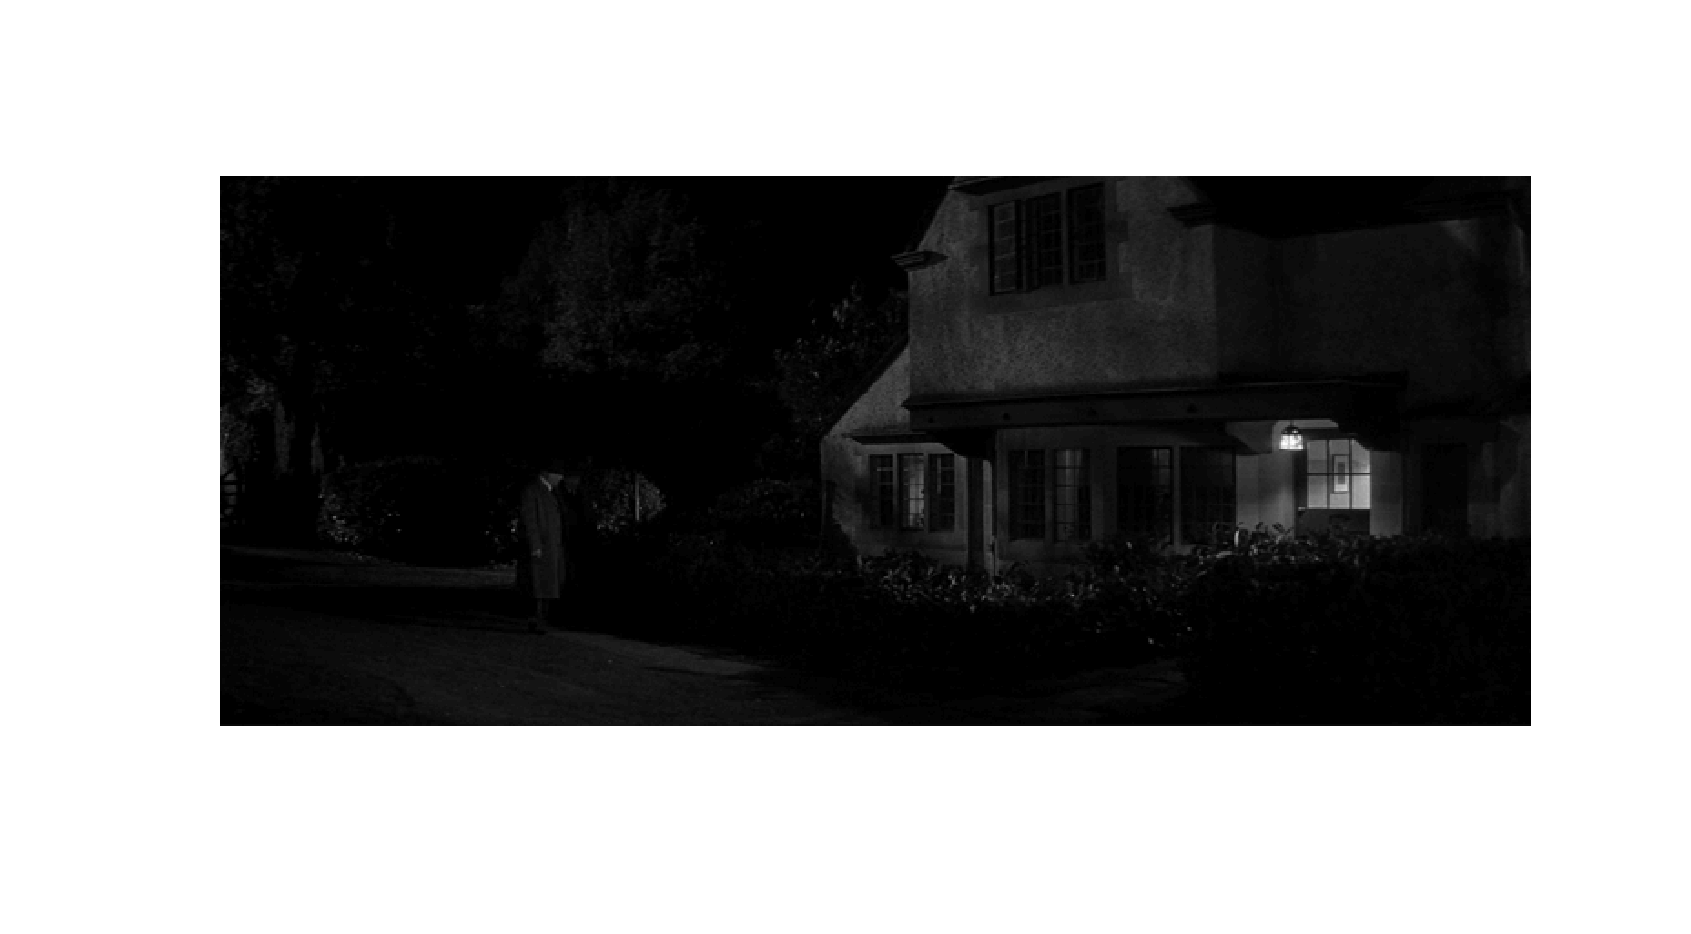
\includegraphics[width=1.0\textwidth]{result_orig_shadowlands}%
			\label{fig:im_orig_ace}%
		}\qquad%
		\subfloat[\emph{ACE}]{%
			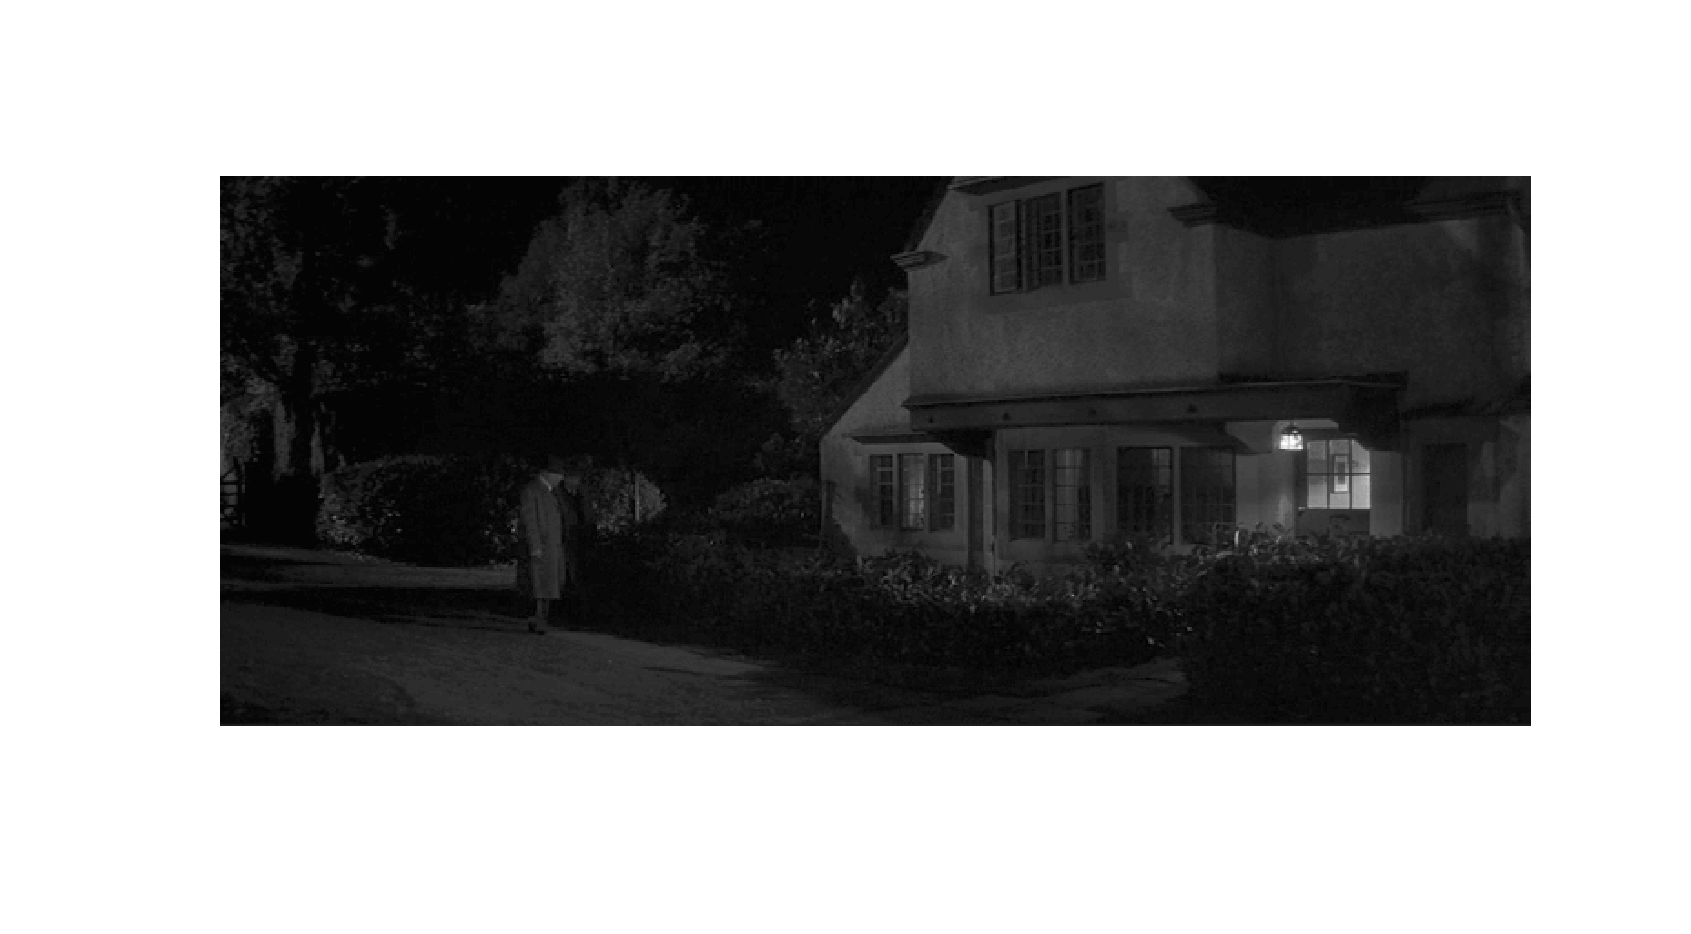
\includegraphics[width=1.0\textwidth]{result_ace_shadowlands}%
			\label{fig:im_ace_ace}%
		}
	\caption{\emph{Comparación entre imágenes con y sin ACE denotando una mejora de contraste entre los objetos.}}
\end{minipage}
